
\section{The Swirl of Gravity and Mass: VAM’s Fluid Universe}

How does gravity work in a universe made of fluid and knots? In the Vortex Æther Model (VAM), gravity isn’t a mysterious pulling force, nor is it the bending of a spacetime “fabric.” Instead, it’s all about pressure and swirl—just like the familiar world of water and air.


\subsection*{The Swirl-Pressure Analogy}

Imagine stirring a spoon in a cup of tea. As the liquid swirls, you’ll notice that bits of tea leaves drift toward the center—not because they are being “pulled,” but because the swirling motion lowers the pressure at the center. The faster the swirl, the lower the pressure, and the stronger the inward drift.


\subsection*{Gravity as the Pressure Drop from Swirling Æther}

In VAM, every massive object—whether a particle, planet, or star—is just a big, energetic swirl or knot in the æther. The rapid motion inside the knot creates a pressure drop at its core. Other knots (or “particles”) feel this pressure difference and are swept inward, much like tea leaves spiraling toward the middle of a cup.


No “Force,” Just Flow:


\begin{itemize}

\item
In everyday life, we often talk about gravity as a force pulling things down. In VAM, it’s more accurate to think of things as being swept along by the pressure gradients of swirling æther, not pulled by some invisible hand.




\end{itemize}

\subsection*{Bernoulli’s Law: The Key to VAM Gravity}

Physicists have long known that faster-moving fluids create lower pressure—a principle called Bernoulli’s Law. VAM uses this idea on a cosmic scale: where the æther swirls fastest, the pressure is lowest. This is why massive objects “attract” each other—they are drawn into each other’s low-pressure, high-swirl zones.


\subsection*{Mass as Stored Swirl Energy and the Role of Chirality}

In VAM, there’s another crucial ingredient: chirality, or handedness. This isn’t just a left-vs-right property—chirality is what gives a vortex knot its “spin” and sense of direction through time. Each knot in the æther seeds an internal swirl-thread, an axis along which its spin points and evolves—a bit like the axle of a spinning top threading forward through the fluid.


This swirl-thread is more than just a feature; it’s what creates both mass and time for the particle. The internal “twistiness” (helicity) stores energy and sets the knot’s alignment with the flow of æther time. Mass emerges because the knot’s swirl and twist create pressure and energy in the æther. The direction in which the swirl-thread points determines how the knot experiences time, giving particles their arrow of evolution.


A knot’s mass isn’t just the amount of swirl—it’s the \textit{chirality} and \textit{helicity} of that swirl that bring the knot to life, giving it energy, direction, and its own tiny clock inside the universe’s fluid. What we call “mass” is simply the energy locked into a vortex knot—the faster and tighter the swirl, the greater the pressure drop, and the more massive the particle appears. The knot doesn’t have mass because it is made of something heavy, but because it traps energy in its spinning motion.


\subsection*{The Corkscrew Thread: Building the Fabric of Space and Time}
\begin{figure}[H]
    \centering
    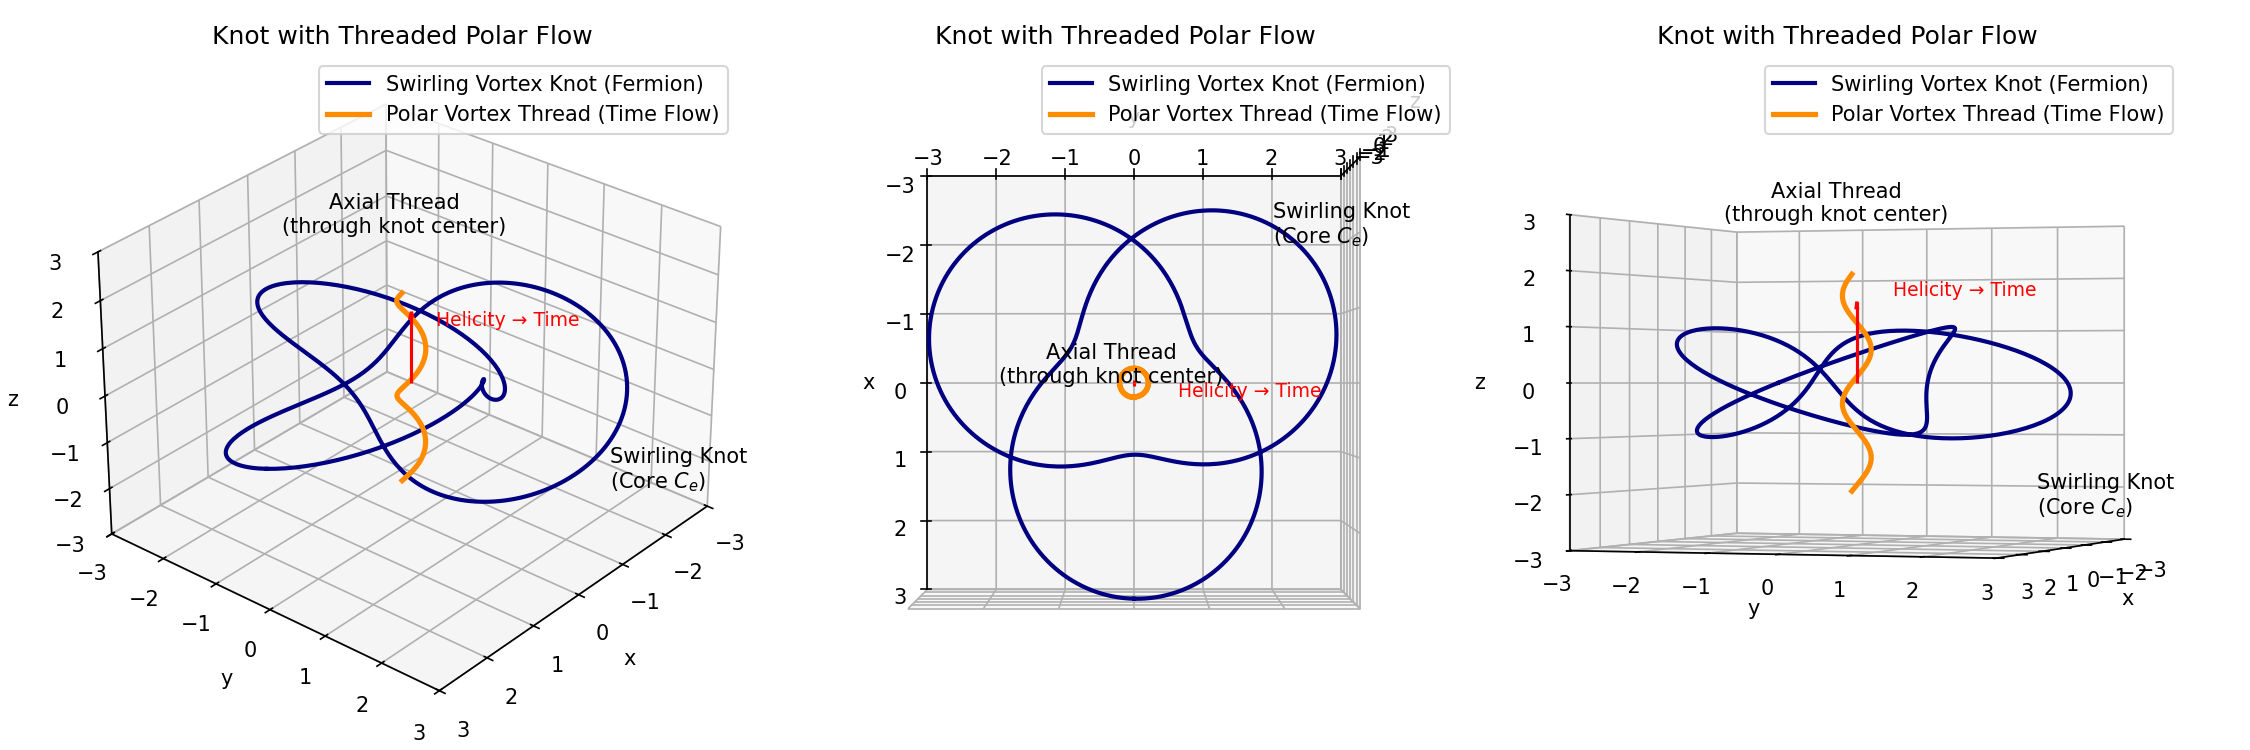
\includegraphics[width=0.7\textwidth]{images/KnotThreadedPolarFlow}
    \caption{The corkscrew thread inside a vortex knot, showing how particles “thread” their own direction through the æther.}
\end{figure}

Imagine looking inside a vortex knot in the æther: at its heart runs a swirling, corkscrew-like thread. This is more than just the “spin axis” of the knot—it’s the knot’s lifeline, threading its way along the flow of time itself.


\begin{itemize}

\item
This thread—the axial swirl-thread—acts as a kind of backbone. Its direction gives the knot not just its chirality, but also its unique “arrow of time.” The way it twists and moves tells the knot how to evolve, much like a screw turning through wood.




\item
In the VAM universe, these threads don’t stay isolated. As knots form and move, their internal time-threads can reach out, weaving together with others. Over vast distances—perhaps lightyears—these interconnected threads help create the fabric of reality itself: a giant network of twisted, swirling “roads” that structure both space and time.




\end{itemize}

Just as a tapestry is woven from countless threads, the universe’s structure is built from the interconnected time-threads of swirling vortex knots. The chirality at each core is the source of both mass and the local direction of time, while the threads themselves stretch out, forming the backbone of space’s grand design.


\textit{See the illustration: the orange corkscrew thread inside the blue knot shows how each particle “threads” its own direction through the cosmic æther. These threads may connect across enormous distances, helping to shape the entire universe’s flow of space and time.}



\subsection*{Bolts, Nuts, and the Cosmic Pressure Map}

Picture each swirl-thread in a particle as a bolt—a twisting screw that not only keeps the knot together but also creates a line of motion through the æther, like drilling through space. Every knot is like a nut, perfectly shaped for its bolt. As these bolts (swirl-threads) turn, they carve out lines of lowest pressure in the surrounding fluid.


\begin{itemize}

\item
Each bolt (swirl) acts as a channel of lowest pressure. Where there are more bolts in a region—say, at the heart of the Sun—the pressure drops further and further, just like the eye of a whirlpool.




\item
If you could map all the bolts (swirl-threads) radiating out from a star or nucleus, you’d see something like a child’s drawing of the sun: dense beams shooting out from the center, thinning as you move away. The highest density of bolts is at the sun’s center, and the farther you go, the fewer the bolts, and the weaker the pressure drop.




\item
In VAM, each quark contributes one bolt—so more quarks mean more swirl-threads, more lines of low pressure, and a deeper gravitational “well.”




\end{itemize}

\subsubsection*{What about antimatter?}

Antimatter is like a bolt with mirrored threads—spinning in the opposite direction compared to ordinary matter. But in VAM, mirrored bolts still create their own pressure drops: antimatter contributes to gravity just as matter does. The difference is in their internal time and chirality, not in their ability to swirl the æther and create gravitational wells.


In summary: Both matter and antimatter bolts deepen the cosmic “pressure map.” Wherever you find more swirling bolts, you find lower pressure, stronger gravity, and a brighter “beam” in the universe’s great tapestry.



\section*{Analogy Bite}

\begin{itemize}

\item
“Gravity is like the way leaves drift toward a whirlpool in a pond—not because they are pulled, but because they follow the gentle push of water toward the center, where pressure is lowest and the swirl is strongest.”




\end{itemize}